En este capítulo se muestran los trabajos relacionados al proyecto propuesto
 en este documento y una breve descripción de estos, se podrá observar una
 diferencia temática entre la temática de los trabajos mostrados; empezando 
 por aquellos que tienen por objetivo ayudara a los discapacitados, 
 posteriormente los trabajos cuyo objetivo es que un robot mecánico o virtual 
 realice tareas de manera similar a como las haría un ser humano y finalmente 
 se muestran métodos para trabajar con datos categóricos, de manera más 
 específica, datos nominales, ya que se contempla desarrollar un clasificador 
 no supervisado de datos nominales.

Las Opciones de accesibilidad de Microsoft Windows han permitido que su
 sistema operativo sea posible usarlo sin importar las condiciones físicas del
 usuario \cite{DanielHubbell2016}. A continuación, se menciona una breve 
 descripción de estas opciones.

\begin{itemize}
	\item Lupa: Aumenta el tamaño del contenido de la pantalla para que sea más
	 fácil leerlo \cite{xatakaaccesiblilidad}.
	\item Narrador:  Esta función es una ayuda auditiva que ayuda a saber cuáles
	 son las ventanas abiertas y su contenido, por medio de una voz sintetizada
	 \cite{xatakaaccesiblilidad}.
	\item Teclado en pantalla: Como su nombre lo indica es un teclado virtual
	 con el cual podemos escribir presionando la pantalla, en caso de ser un
	 dispositivo táctil, o presionando los botones con el ratón
	 \cite{xatakaaccesiblilidad}.
	 \item Contraste alto: Otra ayuda visual para poder distinguir mejor los
	  elementos en pantalla modificando el contraste de Windows
	  \cite{xatakaaccesiblilidad}.
	  \item Reconocimiento de voz: Es una herramienta de dictado con la cual se
	   puede escribir y manipular aplicaciones e incluso el mismo sistema
	   operativo por medio de comandos de voz \cite{support14213}.
\end{itemize}
	   
Aunque no esta considerado dentro de las opciones de accesibilidad de Windows,
 el asistente Cortana facilita la realización de algunas tareas por medio de
 comandos de voz, por ejemplo, apertura de programas, la manipulación de
 recordatorios, mensajes de texto y correo electrónico \cite{support17214}. 

Los archivos por lotes (Batch o Script Shell) \cite{Silberschatz1999} son
 archivos que contienen instrucciones para el sistema operativo en formato
 ASCII por lo que son dependientes de él, por lo general tienen la extensión
 .bat o .sh, sin embargo, para el caso de UNIX esto no es obligatorio. En la
 imagen~\ref{fig:script} se muestra el código de un archivo por lotes y la 
 ejecucion en consola.


\begin{figure}[H]
\centering
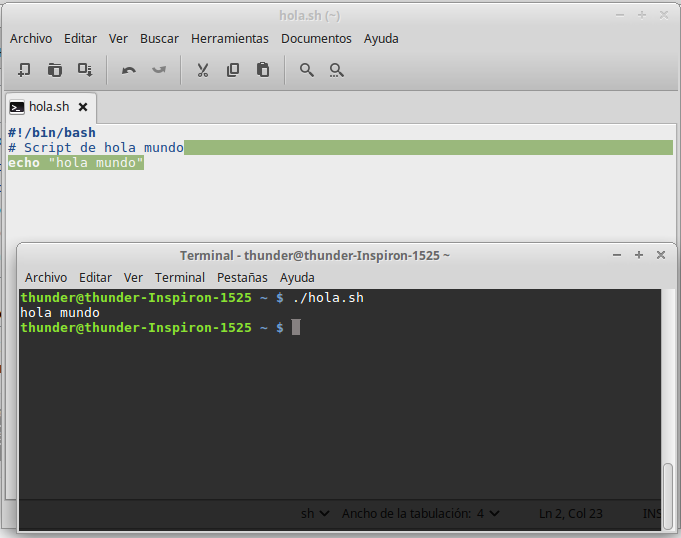
\includegraphics[width=0.7\columnwidth]{CapituloI/Imagenes/Script.png}
\caption{Ejecución de un archivo por lotes en Linux.}
\label{fig:script}
\end{figure}


Pulover's Macro Creator\cite{Batista}, desarrollado y mantenido
 principalmente por Rodolfo U. Batista, es una herramienta de automatización
 y creación de scripts basada en el lenguaje ``AutoHotKey''. Este creador de
 macros facilita la tarea de la creación del script por medio de su interfaz
 gráfica ó con la grabadora de macros que proporciona. Entre sus
 características destaca el proporcionar control de ventanas en segundo plano
 y sentencias de control(ciclos y condicionales). En la imagen
 ~\ref{fig:macros} se puede observar la interfaz de usuario del software.


\begin{figure}[H]
\centering
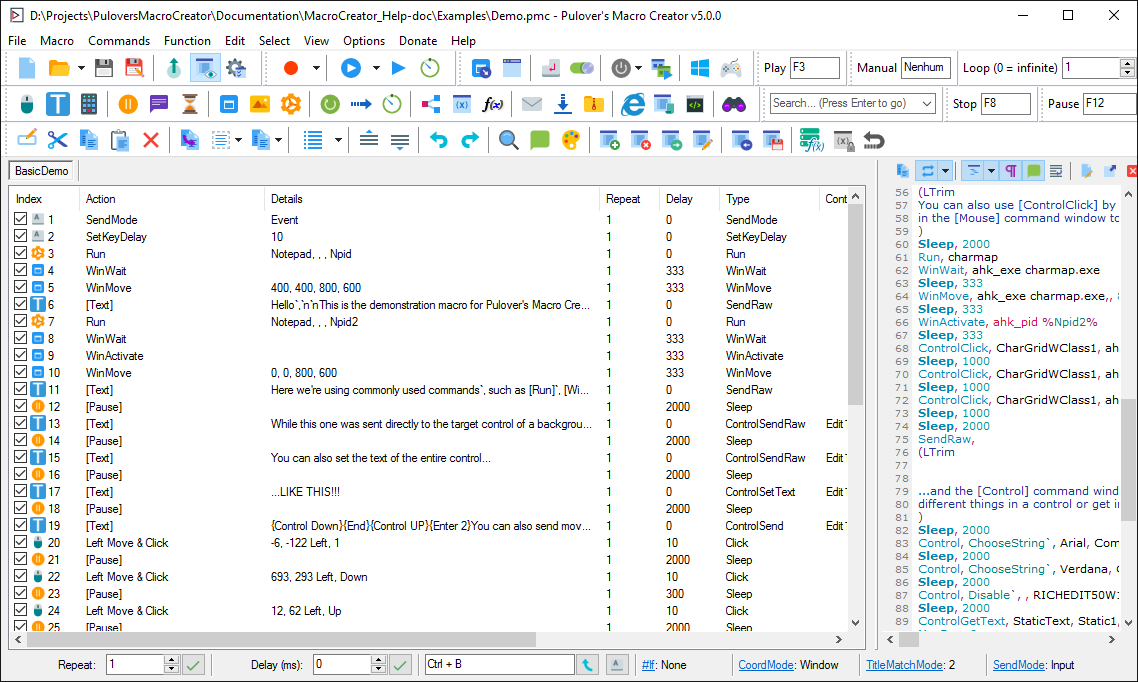
\includegraphics[width=0.7\columnwidth]{CapituloI/Imagenes/Macros.png}
\caption{Interfaz de usuario de Pulover's Macro Creator con una macro de
 ejemplo.}
\label{fig:macros}
\end{figure}



Un trabajo desarrollado por la Universidad de Tsukuba en
 Japón\cite{Nakano2006}, tiene por objetivo el crear un oponente virtual
 al nivel de un oponente humano que represente un reto para el jugador. Para
 lograr esto se crearon perfiles con las estrategias de los jugadores y
 posteriormente se reproducen en otra partida, en la imagen~\ref{fig:imitat}
 se muestra el entorno del juego.


\begin{figure}[H]
\centering
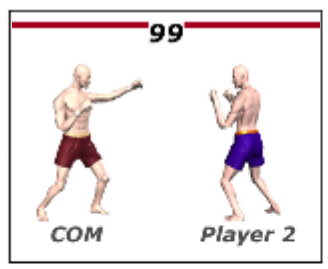
\includegraphics[width=0.5\columnwidth]{CapituloI/Imagenes/Imitating.png}
\caption{Ambiente del juego de acción.}
\label{fig:imitat}
\end{figure}


En el trabajo desarrollado en la Universidad Tecnológica de Lanzhou en China
 \cite{Zhang2017},hacen un análisis del comportamiento del soldador experto
 humano utilizando un sistema de inferencia neurodifuso adaptativo (ANFIS,
 por sus siglas en inglés) para su automatización, considerando las variables
 de los materiales usados y caracterizando la tarea del soldador humano.
 En la imagen~\ref{fig:syswelding} se puede apreciar el sistema experimental
  resultante del proyecto mencionado.


\begin{figure}[H]
\centering
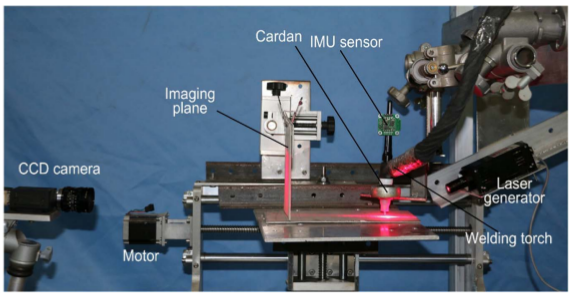
\includegraphics[width=0.8\columnwidth]{CapituloI/Imagenes/Welding.png}
\caption{Sistema experimental de la soldadora.}
\label{fig:syswelding}
\end{figure} 
 

En el ambiente artístico \cite{Nishiguchi2017}, el trabajo desarrollado en
 Japón por la Universidad de artes de Tokyo y la Universidad de Osaka, cuyo
 objetivo era brindar un comportamiento natural humano a un Robot Humanoide.
 Para cumplir esto utilizaron el conocimiento del director de escena Hirata,
 que dada la precisión en sus instrucciones a los actores, facilita la
 traducción de esas órdenes a las reglas para el robot humanoide, además,
 desarrollaron una interfaz de usuario para que el manejo del robot sea más
 sencillo, ayudando a los principiantes, ya que proporcionan menos datos se
 puede obtener buenos resultados. Como se puede observar en la imagen
 ~\ref{fig:theatricalrob} el robot llego a desempeñar un amigo del
 personaje principal en la obra ``Night on the milky way train''
 (El tren nocturno de la vía láctea) en un escenario real.


\begin{figure}[H]
\centering
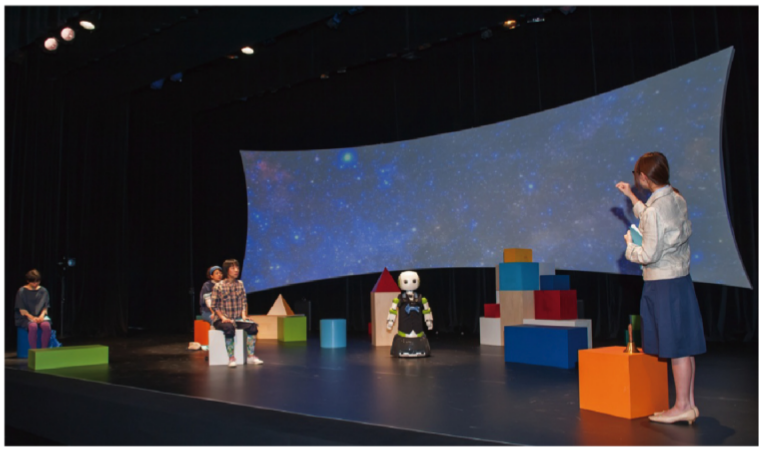
\includegraphics[width=0.8\columnwidth]{CapituloI/Imagenes/Theatrical.png}
\caption{Robot humanoide actor en escenario real.}
\label{fig:theatricalrob}
\end{figure} 


El trabajo desarrollado por la Universidad de Plymouth, Universidad de
 Lincoln ambas en el Reino Unido y la Universidad de Gante en Bélgica
 \cite{Senft2016}, realiza un análisis comparativo de su método SPARC (Supervised
 Progressively Autonomous Robot Competencies) con el IRL (Interactive
 Reinforcement Learning), estos dos métodos se basan en el aprendizaje 
 automático de un robot, haciendo que un ser humano con conocimiento del tema
 apruebe la actividad que está realizando o que va a realizar el robot.
 Ambos sistemas fueron probados en un ambiente virtual nombrado ``sophie’s
 kitchen''(La cocina de Sofia) cuyo objetivo es hornear un pastel, 
 la imagen ~\ref{fig:sparcrob} muestra al robot en la cocina con los materiales
 necesarios para realizar la tarea. 
 
\begin{figure}[H]
\centering
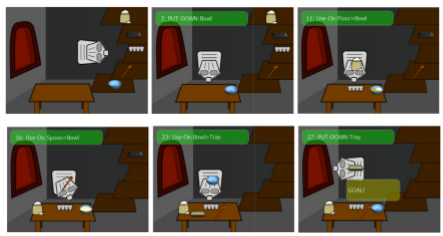
\includegraphics[width=0.8\columnwidth]{CapituloI/Imagenes/Sparc.png}
\caption{Robot virtual en “sophie’s kitchen”(La cocina de Sofia).}
\label{fig:sparcrob}
\end{figure}


El trabajo realizado en la Universidad Nacional Chiao Tung y el Instituto
 Politécnico Kaohsiung ambos en Taiwán\cite{Chang1996}, propone un algoritmo
 que imite el comportamiento del aprendizaje humano como una solución al
 aprendizaje automático en ambientes imperfectos, por ejemplo, cuando la
 información esta incompleta. Este algoritmo demuestra en los experimentos
 realizados ser superior al algoritmo ID3 y PRISM.